% Author:  Brad Burkman
% Date:  21 August 2018
% Notes for Fall 2018 CSCE 515
%	Principles of Computer Graphics
%	Dr. Christoph Borst

\documentclass[12pt]{article}
\usepackage{tikz}
\usetikzlibrary{arrows, calc}
\usepackage{pgfmath}
\usepackage{setspace}
\usepackage{amsmath}
\usepackage{array}
\usepackage{hyperref}
\usepackage{color}
\setlength{\pdfpageheight}{11in}
\setlength{\textheight}{9in}
\setlength{\voffset}{-1in}
\setlength{\oddsidemargin}{0pt}
\setlength{\marginparsep}{0pt}
\setlength{\marginparwidth}{0pt}
\setlength{\marginparpush}{0pt}
\setlength{\textwidth}{6.5in}

\pagestyle{empty}
\begin{document}
\setlength{\parindent}{0pt}
\begin{spacing}{1.2}

%%%%
%
%  Put the name of your main file in the brackets after "\input" below.
%
%%%%%

Brad Burkman's Notes for

\qquad CSCE 515 Principles of Computer Graphics

\qquad Dr. Christoph Borst, CBDI co-PI, 
OLVR 342, 
\url{cbx99999@louisiana.edu}

\qquad Fall 2018

\

Grader:  Jason Woodworth, \url{downtothelastpixel@gmail.com}

\tableofcontents

%%%%%%%%%%%%
\section{Classmates}
%%%%%%%%%%%%

Generally where people sit:  (Please correct)

\begin{tabular}{lllll}
	Andrew Young & Laura Charney & Kim Smith \cr
	Sergio Hernandez & Marcus Shannon & Lou Landry-Linet & Brad Burkman & Anna Kovalenko \cr
	& Ryan Stelly \cr
	Yitoshee Rahman & Alex Talley & Andrew Young & Kayzleigh Prejean \cr
	Benjamin Yerino & Aaron Wiley & Joey Maquin \cr
\end{tabular}

\

Not on the chart.  Please correct the chart.  

Mark Kimble

Andre Longon

Jason Woodworth

Yihe Zhang

Davis Garrett

Karly Wilson

Connor Lambert

Brock Landry

Brock Comeaux

Somtoo Charles Chukwu

Ege Beyazit

Sarker Monogit Asish

\


%%%%%%%%%%%%
\section{Tuesday 21 August:  Introduction}
%%%%%%%%%%%%%

Ray Tracing

OpenGL 3.3

\qquad Couldn't find a textbook that did both the math and OpenGL 3.3 well.  

Cross Product v/s Dot Product of Vectors

Start with how lines and triangles are rendered.  

Acknowledge sources I used in homework and projects.  

Exam will be hard.  

Lagniappe - Come to VR lab to do a project.  

\

%%%%%%%%%%%%
\section{Math Review:  Dot Product and Cross Product}
%%%%%%%%%%%%%

Example of Dot Product and Cross Product:

$\vec{u} = \langle 1,2,3 \rangle$

$\vec{v} = \langle 4,5,6 \rangle$

\

$\vec{u} \cdot \vec{v} = 1 \cdot 4 + 2 \cdot 5 + 3 \cdot 6 = 4 + 10 + 18 = 32$

\

$\displaystyle \vec{w} = \vec{u} \times \vec{v} = 
	\left|
	\begin{tabular}{*3{>{$}c<{$}}}
		\vec{i} & \vec{j} & \vec{k} \cr
		1 & 2 & 3 \cr
		4 & 5 & 6 \cr
	\end{tabular}
	\right|
\ = \
	\left|
	\begin{tabular}{cc}
		2 & 3 \cr
		5 & 6 \cr
	\end{tabular}
	\right|
	\vec{i}
\ - \	
	\left|
	\begin{tabular}{cc}
		1 & 3 \cr
		4 & 6 \cr
	\end{tabular}
	\right|
	\vec{j}
\ + \ 
	\left|
	\begin{tabular}{cc}
		1 & 2 \cr
		4 & 5 \cr
	\end{tabular}
	\right|
	\vec{k}
\ = \
	-3\vec{i} + 6 \vec{j} - 3 \vec{k}
\ = \
	\langle -3,6,-3 \rangle
$

\

Is the cross product commutative?

\

$\displaystyle\vec{v} \times \vec{u} = 
	\left|
	\begin{tabular}{*3{>{$}c<{$}}}
		\vec{i} & \vec{j} & \vec{k} \cr
		4 & 5 & 6 \cr
		1 & 2 & 3 \cr
	\end{tabular}
	\right|
\ = \
	\left|
	\begin{tabular}{cc}
		5 & 6 \cr
		2 & 3 \cr
	\end{tabular}
	\right|
	\vec{i}
\ - \	
	\left|
	\begin{tabular}{cc}
		4 & 6 \cr
		1 & 3 \cr
	\end{tabular}
	\right|
	\vec{j}
\ + \ 
	\left|
	\begin{tabular}{cc}
		4 & 5 \cr
		1 & 2 \cr
	\end{tabular}
	\right|
	\vec{k}
\ = \
	3\vec{i} - 6 \vec{j} + 3 \vec{k}
\ = \
	\langle 3,-6,3 \rangle
\ = \ -\vec{w}
$

\

No, it's anti-commutative, but that's okay.  The cross product gives a vector, $\vec{w}$, orthogonal to both $\vec{u}$ and $\vec{v}$, and a constant multiple of $\vec{w}$ is still orthogonal to both other vectors.  

\

The cross product is also not associative, but satisfies the Jacobi identity.

$$a \times (b \times c) + b \times (c \times a) + c \times (a \times b) = 0 \ \forall a, b, c \in V$$

%%%%%%%%%%%%%%%%
\section{Math Review:  Algebra}
%%%%%%%%%%%%%%%%%%

A {\bf group} is a set $S$ with an operation (``+'')  such that:

\qquad The set S is {\it closed} under the operation, meaning that if $a,b \in S$, then $a+b \in S$.

\qquad The operation is associative, meaning that if $a,b,c \in S$, then $a+(b+c) = (a+b)+c$.

\qquad The set $S$ contains a unit element (``0''), such that $a+0 = 0+a = a \ \forall \ a \in S.$

\qquad For every element $a \in S$, there is an inverse element, $-a$, such that $a+(-a) = -a + a = 0$.

If the operation is commutative, meaning $a+b = b+a \ \forall \ a, b, \in S$, then $S$ is called an {\bf Abelian group.}

\

A {\bf ring} is a set $R$ with two operations, $+$ and $\cdot$, such that:

\qquad The set $R$ is an Abelian group.  

\qquad The set $R$ is closed under multiplication.

\qquad Multiplication is associative.  

\qquad The distributive laws hold:

\qquad \qquad $a \cdot (b+c) = a \cdot b + a \cdot c$

\qquad \qquad $(b+c) \cdot a = b \cdot a + c \cdot a$

A ring with a multiplicative identity (``1'') is called a {\bf ring with unit}.

If the ring has the property that if $a\cdot b = 0$ then $a=0$ or $b=0$, it is called a {\bf domain}.

If multiplication is commutative, then the ring is called a {\bf commutative ring}.

If a domain is commutative, then it is called an {\bf integral domain}.

\

A {\bf field} is a commutative ring with unit element (``1'') such that every nonzero element has an inverse.  

\

Quaternions are not a field because multiplication of quaternions is not commutative; however, every nonzero quaternion has a multiplicative inverse, so they are called a {\bf division ring}.

%%%%%%%%%
\section{Math Review:  Quaternions}
%%%%%%%%%%%

Complex numbers, $a+bi$ where $a$ and $b$ are real numbers and $i = \sqrt{-1}$, are two-dimensional numbers.  Quaternions, $a + bi + cj + dk$, are four-dimensional numbers.  Just as you can think of complex numbers being two-dimensional vectors having the basis vectors $1 = \langle 1,0 \rangle$ and $i = \langle 0,1 \rangle$, you can think of quaternions as four-dimensional vectors having the basis vectors 
$1 = \langle 1,0,0,0 \rangle$, 
$i = \langle 0,1,0,0 \rangle$, 
$j = \langle 0,0,1,0 \rangle$, 
$k = \langle 0,0,0,1 \rangle$, 

\

While complex numbers have the basis elements 1 and $i$ with, $i^2 = -1$, quaternions have this multiplication scheme for their basis elements.  Note that $i^2 = j^2 = k^2 = ijk = -1$, but they are anti-commutative, with, for example, $ij = -ji$.

\

\hfil\begin{tabular}{*5{>{$}c<{$}|}}
	\times & 1 & i & j & k \cr \hline
	1 & 1 & i & j & k \cr \hline
	i & i & -1 & k & -j \cr \hline
	j & j & -k & -1 & i \cr \hline
	k & k & j & -i & -1 \cr
\end{tabular}
\hfil
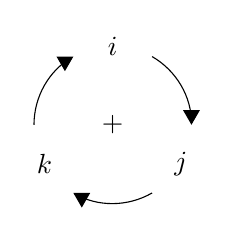
\begin{tikzpicture}[x=10mm, y=10mm]
%	\draw (0,0) circle (1.3);
	\coordinate (I) at (0,1);
	\coordinate (J) at ({cos(-30)},{sin(-30)});
	\coordinate (K) at ({cos(210)},{sin(210)});
	\draw (I) node {$i$};
	\draw (J) node {$j$};
	\draw (K) node {$k$};
	\draw [triangle 60-] (1,0) arc (0:60:1);
	\draw [triangle 60-] ({cos(120)},{sin(120)}) arc (120:180:1);
	\draw [triangle 60-] ({cos(240)},{sin(240)}) arc (240:300:1);
	\draw (0,0) node {$+$};

\end{tikzpicture}
\hfil
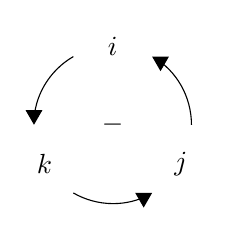
\begin{tikzpicture}[x=10mm, y=10mm]
%	\draw (0,0) circle (1.3);
	\coordinate (I) at (0,1);
	\coordinate (J) at ({cos(-30)},{sin(-30)});
	\coordinate (K) at ({cos(210)},{sin(210)});
	\draw (I) node {$i$};
	\draw (J) node {$j$};
	\draw (K) node {$k$};
	\draw [-triangle 60] (1,0) arc (0:60:1);
	\draw [-triangle 60] ({cos(120)},{sin(120)}) arc (120:180:1);
	\draw [-triangle 60] ({cos(240)},{sin(240)}) arc (240:300:1);
	\draw (0,0) node {$-$};

\end{tikzpicture}
\hfil

\

The inverse of a quaternion is given by:

$$ (a + bi + cj + dk)^{-1} = \frac{a - bi - cj - dk}{a^2 + b^2 + c^2 + d^2}$$

\

{\bf Vector Form of Quaternions}

Think of $a + bi + cj + dk$ as the pair, $(a, \langle b,c,d \rangle )$, with a scalar part and a vector part.  

Then quaternion addition is \ $(r_1, \vec{v}_1) + (r_2, \vec{v}_2) = (r_1 + r_2, \vec{v}_1 + \vec{v}_2)$.

Vector multiplication is $(r_1,\vec{v}_1) (r_2,\vec{v}_2) = (r_1r_2 - \vec{v}_1 \cdot \vec{v}_2, \ r_1\vec{v}_2 + r_2 \vec{v}_1 + \vec{v}_1 \times \vec{v}_2)$


\subsection{Quaternions as Rotations}

We start with a vector, $\vec{p} = (p_x, p_y, p_z)$, written as a quaternion with real coordinate zero, 
$$p = p_x \mathbf{i} + p_y \mathbf{j} + p_z \mathbf{k}$$

We want a rotation of $p$ through an angle of $\theta$ about the axis defined by a unit vector $$\vec{u} =  ( u_x, u_y, u_z ) = u_x \mathbf{i} + u_y \mathbf{j} + u_z \mathbf{k}$$ 

In two dimensions, Euler's Formula,  $e^{i\theta} = \cos \theta + i \sin \theta$, gives a counterclockwise rotation of $\theta$.  We can extend it to three dimensions as
$$q = e^{ 
	\frac{\theta}{2}
	( u_x \mathbf{i} + u_y \mathbf{j} + u_z \mathbf{k} )
	}
=
	\cos \frac{\theta}{2} + ( u_x \mathbf{i} + u_y \mathbf{j} + u_z \mathbf{k} ) \sin \frac{\theta}{2}
$$

The rotation of $\vec{p}$ about $\vec{u}$ is given by 
$$p' = q p q^{-1}$$

Going back to using Euler's Formula for a rotation, let's look at the multiplicative inverse of $q$ and see that it's consistent with previous knowledge.  By a previous formula, 
$$a^{-1} = (a_w + a_x \mathbf{i} + a_y \mathbf{j} + a_z \mathbf{k})^{-1} = 
\frac{1}{a_w^2 + a_x^2 + a_y^2 + a_z^2} (a_w - a_x \mathbf{i} - a_y \mathbf{j} - a_z \mathbf{k} )$$

The vector $\vec{u} = u_x \mathbf{i} + u_y \mathbf{j} + u_z \mathbf{k}$ is a unit vector with real part zero, so the denominator is 1.  
$$(\vec{u})^{-1} = (u_x \mathbf{i} + u_y \mathbf{j} + u_z \mathbf{k})^{-1} = -u_x \mathbf{i} - u_y \mathbf{j} - u_z \mathbf{k} = -\vec{u}$$

Applying the extension of Euler's Formula, 
$$q = e^{ 
	\frac{\theta}{2}
	( u_x \mathbf{i} + u_y \mathbf{j} + u_z \mathbf{k} )
	}
=
	\cos \frac{\theta}{2} + ( u_x \mathbf{i} + u_y \mathbf{j} + u_z \mathbf{k} ) \sin \frac{\theta}{2}
$$

and the inverse formula

$$a^{-1} = (a_w + a_x \mathbf{i} + a_y \mathbf{j} + a_z \mathbf{k})^{-1} = 
\frac{1}{a_w^2 + a_x^2 + a_y^2 + a_z^2} (a_w - a_x \mathbf{i} - a_y \mathbf{j} - a_z \mathbf{k} )$$

we get

$$q^{-1} = \frac{1}{
	\cos^2 \frac{\theta}{2}
	 + u_x^2 \sin ^2 \frac{\theta}{2}
	 + u_y^2 \sin ^2 \frac{\theta}{2}
	 + u_z^2 \sin ^2 \frac{\theta}{2}
	}
	\left(\cos \frac{\theta}{2} - ( u_x \mathbf{i} + u_y \mathbf{j} + u_z \mathbf{k} ) \sin \frac{\theta}{2}\right)
$$

$$ = \frac{1}{
	\cos^2 \frac{\theta}{2}
	 + (u_x^2 
	 + u_y^2 
	 + u_z^2) \sin ^2 \frac{\theta}{2}
	}
	\left(\cos \left( - \frac{\theta}{2} \right) + ( u_x \mathbf{i} + u_y \mathbf{j} + u_z \mathbf{k} ) \sin \left(-\frac{\theta}{2}\right)\right)
$$

$$ = \frac{1}{
	\cos^2 \frac{\theta}{2}
	+ \sin ^2 \frac{\theta}{2}
	}
	\left(\cos \left( - \frac{\theta}{2} \right) + ( u_x \mathbf{i} + u_y \mathbf{j} + u_z \mathbf{k} ) \sin \left(-\frac{\theta}{2}\right)\right)
$$

$$ = e^{\frac{\theta}{2}(-u)} = \left(e^{\frac{\theta}{2}u}\right)^{-1}
$$

%%%%%%%%%%%%%%%%
\section{Thursday 23 August:  Raster Display v/s Vector Display}
%%%%%%%%%%%%%%%%%

\

{\bf Ray Tracing}:  Which objects intersect the line?

\

{\bf Polygon Projection (Polygon Rendering)}

Triangles on the screen

Vertex coordinates

Multiply by matrices to convert to screen's coordinate system

\

Modeling Coordinates 

\qquad $\to$ World Coordinates

\qquad $\to$ Viewing and Projection Coordinates (Camera View)

\qquad $\to$ Normalized Coordinates

\qquad $\to$ Device Coordinates

\

\begin{tabular}{m{0.3in}m{.2in}*4{m{1.0in}m{.2in}}}
	$\left[ \begin{matrix} x \cr y \cr z \cr w \cr \end{matrix}\right]$
	&
	$\to$
	&
	Model \par Martrix
	&
	$\to$
	&
	Projection \par Matrix \par (Camera View)
	&
	$\to$
	&
	Perspective \par Division
	&
	$\to$
	&
	Viewpoint \par Transformation
	\cr
\end{tabular}

\

{\bf 2D Scan Conversion}:  Converts 2D object description to pixel values. 

{\it ``Pixel''}  Picture Element

Visible Surface Determination:  Occlusion

\

Direct Illumination v/s Global Illumination:  Shadows not completely dark

Curves and surfaces give a smooth alternative to polygonal representation of objects.  

\

Lots of student projects have dealt with {\bf Particle Dynamics}

\

{\bf Early Video Games}  Nimatron (1940)  First ``video'' game used an oscilloscope as its screen.  

\

{\bf Raster Display} - Image broken into pixels

{\bf Vector Display} - Smooth curves, like moving lasers or electron beam.  

\

Black \& white {\bf bitmap} has one bit per pixel

\

{\bf Raster Displays}

More computationally expensive

Requires more memory

Constant refresh rate

Supports area fills

Won over vector after memory got cheap.  

\

Frame buffers are getting more complex.  

\qquad Double buffering so screen doesn't refresh in the middle of a memory move

\qquad Left and right buffers for stereoscopic rendering

\qquad Depth buffer for occlusion

\

{\bf Know from Today's Lesson}

Pixel, raster, bitmap, frame buffer, {\it aliasing}

Know the difference between raster and vector.  

\

{\bf Aliasing} - in computer graphics, the jagged, or saw-toothed appearance of curved or diagonal lines on a low-resolution monitor.

%%%%%%%%%%%%%%
\section{Tuesday 28 August:  Scan Conversion of a Line Segment}
%%%%%%%%%%%%%%%%

{\bf Simplifying Assumptions}

1-pixel-thick line on a B\&W display (monochrome)

$m \in [-1,1]$.  More elaborate code can deal with other slopes.

Line segment described by two integer endpoints (endpoints fall exactly on pixels) $(x_s,y_s), (x_e,y_e)$

\

\hfil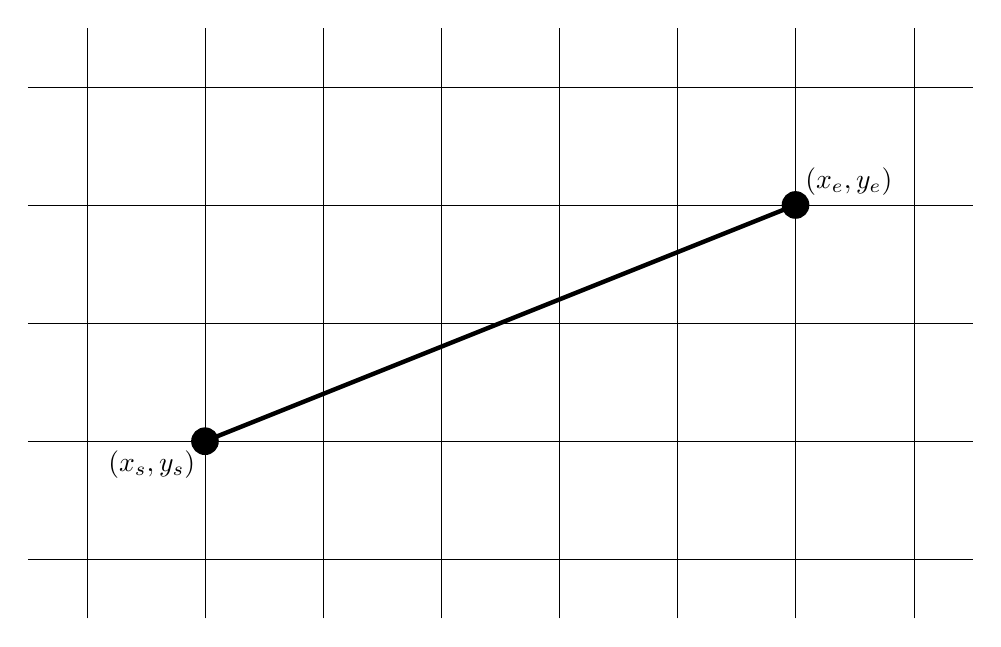
\begin{tikzpicture}[x=15mm, y=15mm]
	\foreach \i in {0,1,2,...,4}{
		\draw [ultra thin] (-0.5,\i) -- (7.5,\i);
	}
	\foreach \i in {0,1,2,...,7}{
		\draw [ultra thin] (\i,-0.5) -- (\i,4.5);
	}
	\coordinate (S) at (1,1);
	\coordinate (E) at (6,3);
	\fill (S) circle (5pt) node [below left] {$(x_s,y_s)$};
	\fill (E) circle (5pt) node [above right] {$(x_e,y_e)$};
	\draw [ultra thick] (S) -- (E);
\end{tikzpicture}

{\bf Main Idea}:  Activate one pixel per column from $x_s$ to $x_e$.  

\

\hfil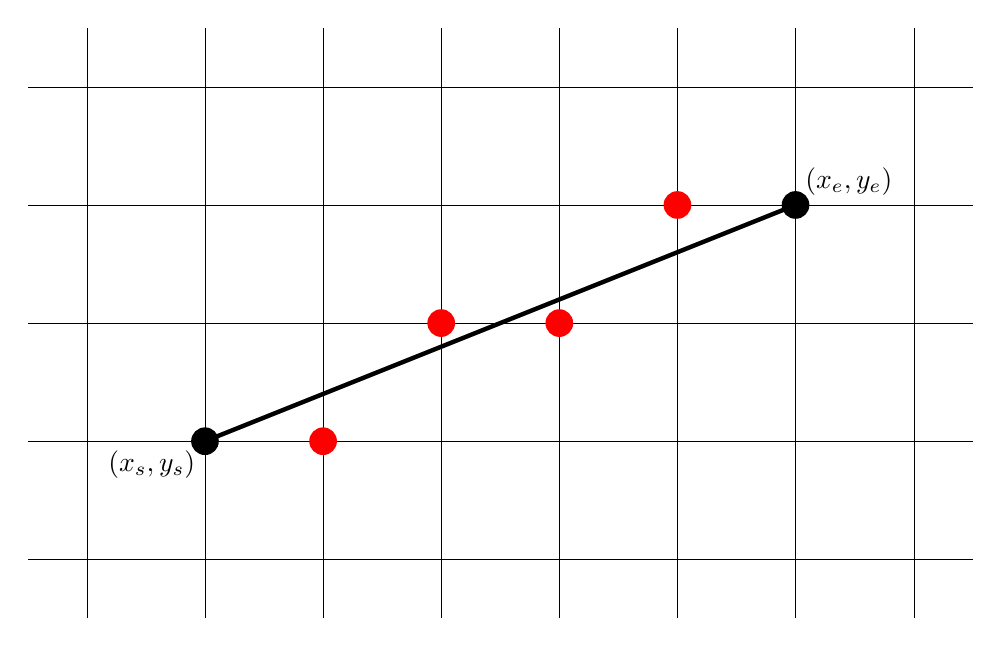
\begin{tikzpicture}[x=15mm, y=15mm]
	\foreach \i in {0,1,2,...,4}{
		\draw [ultra thin] (-0.5,\i) -- (7.5,\i);
	}
	\foreach \i in {0,1,2,...,7}{
		\draw [ultra thin] (\i,-0.5) -- (\i,4.5);
	}
	\coordinate (S) at (1,1);
	\coordinate (E) at (6,3);
	\fill (S) circle (5pt) node [below left] {$(x_s,y_s)$};
	\fill (E) circle (5pt) node [above right] {$(x_e,y_e)$};
	\draw [ultra thick] (S) -- (E);
	\fill [red] (2,1) circle (5pt);
	\fill [red] (3,2) circle (5pt);
	\fill [red] (4,2) circle (5pt);
	\fill [red] (5,3) circle (5pt);
\end{tikzpicture}

{\bf Simple, but Slow, Algorithm}

$m = (y_e - y_s) / (x_e - x_s)$

$b = y_s - m \cdot x_s$

for $x$ from $x_s$ to $x_e$ {\color{red} \it (inclusive)}

\qquad color pixel at $(x, \lfloor m \cdot x + b + 0.5 \rfloor)$

\

The problem with this algorithm that is the $m \cdot x$, floating-point multiplication, is really computationally expensive, usually six cycles, while addition is relatively cheap, usually one cycle.  

\

Rendering algorithms have to be as fast as possible, because they run billions of times.  

\

{\bf Basic Incremental Algorithm (DDA, Digital Differential Analyzer)}

$m = (y_e - y_s) / (x_e - x_s)$

$b = y_s - m \cdot x_s$

$x_0 = x_s$

$y_0 = y_s$

for $i$ from 1 to $(x_e - x_s)$

\qquad $(x_{i+1}, y_{i+1}) = (x_i + 1, y_i + m)$

\qquad color pixel at $(x_i+1, \lfloor y_{i+1} + 0.5 \rfloor )$ 

\

{\bf Midpoint Algorithm (Besenham)}

Developed for pen plotter.

Bottleneck was algorithm and computational speed, not hardware speed.

\

Simplifying assumption:  $m \in [0,1]$

\

Main idea

\qquad Move either E or NE in each move.  

\qquad Choose based on value of decision variable, $d$, which lets us choose betwen E and NE.  

\

\

\hfil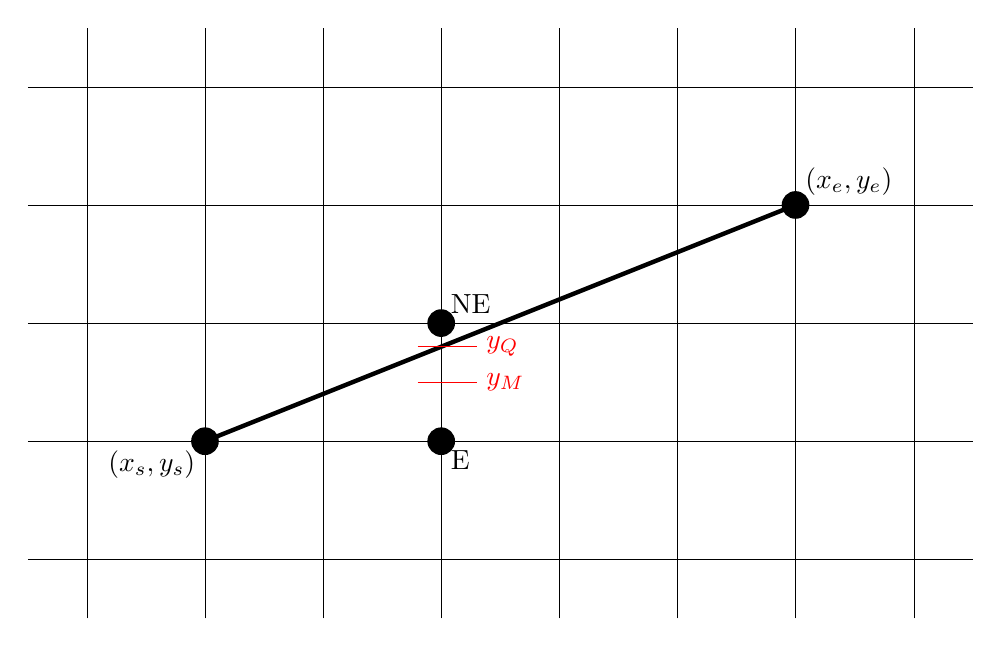
\begin{tikzpicture}[x=15mm, y=15mm]
	\foreach \i in {0,1,2,...,4}{
		\draw [ultra thin] (-0.5,\i) -- (7.5,\i);
	}
	\foreach \i in {0,1,2,...,7}{
		\draw [ultra thin] (\i,-0.5) -- (\i,4.5);
	}
	\coordinate (S) at (1,1);
	\coordinate (E) at (6,3);
	\fill (S) circle (5pt) node [below left] {$(x_s,y_s)$};
	\fill (E) circle (5pt) node [above right] {$(x_e,y_e)$};
	\draw [ultra thick] (S) -- (E);
	\draw [red] (2.8,1.8) -- (3.3,1.8) node [right, red] {$y_Q$};
	\draw [red] (2.8,1.5) -- (3.3,1.5) node [right, red] {$y_M$};
	\fill (3,1) circle (5pt) node [below right] {E};
	\fill (3,2) circle (5pt) node [above right] {NE};
\end{tikzpicture}

Notation:   $Q$ for {\it crossing}, $M$ for {\it midpoint}.

\

{\bf Algorithm}

$d = y_Q - y_M$.  

Look at sign of $d$.  

Move NE when $d$ is positive.

Move E otherwise.  

\

{\bf Computing $d$}

Initialize $d = m - 0.5$

Increment:

\qquad for E moves:  $d = d+m$

\qquad for NE moves:  $d = d + m - 1$

\

Here's how Midpoint is cheaper than DDA:  We can change everything to integers and not have any floats.  

\

{\bf Make Everything Integers}

Scale everything by $2 \Delta x$, so that $m - 0.5$ becomes an integer.  

$d = 2 \Delta y - \Delta x$

East increment:  $d = d + 2 \Delta y$

NE increment:  $d = d + 2 \Delta y - 2 \Delta x$

\

These methods aren't what we use today.  Probably triangle scan conversion.  

%%%%%%%%%
\section{Thursday 30 August:  Scan Conversion of a Triangle}
%%%%%%%%%%%

\subsection{Homework 1} due 13 September

{\it Callback}  Do sth when sth happens

Will have global variables

Assignment is given as a triangle with a certain order of $x_0$, $x_1$, and $x_2$.  Extra part of assignment is to account for different orders.  

\

\subsection{Midpoint Algorithm (Besenham) Pseudocode}

Initialize integers $\Delta_E$, $\Delta_{NE}$, $d$, $x$, and $y$.  

Set pixel at $(x,y)$ (first pixel)

\

{\bf while} $x$ $<$ last column (given by an endpoint)

\{

	\qquad increment $x$ by 1
	
	\qquad {\bf if} ($d<0$)
	
		\qquad \qquad add $\Delta _E$ to $d$
	
	\qquad {\bf else}
	
	\qquad \{
	
		\qquad \qquad increment $y$ by 1
		
		\qquad \qquad add $\Delta_{NE}$ to $d$
	
	\qquad \}
	
	\qquad set pixel at $(x,y)$

\}

\

\subsection{Naming Conventions}

\hfil\begin{tikzpicture}[x=16mm, y=16mm]
	\coordinate (A) at (0,0);
	\coordinate (B) at (-4,4);
	\coordinate (C) at (2,6);
	\draw (A) -- (B) -- (C) -- (A);
	\path (A) node [below] {$(x_0,y_0,R_0,G_0,B_0)$};
	\path (B) node [left] {$(x_1,y_1,R_1,G_1,B_1)$};
	\path (C) node [above] {$(x_2,y_2,R_2,G_2,B_2)$};
	
	\coordinate (M01) at (-2,2);
	\coordinate (L01) at ($(M01) - ({1/sqrt(2)},{1/sqrt(2)})$);
	\node (NM01) at (M01) {};
	\node (NL01) at (L01) {$L_{0,1}$};
	\draw [->] (NL01) -- (NM01);

	\coordinate (M02) at (1,3);
	\coordinate (L02) at ($(M02) + ({3/sqrt(10)},{-1/sqrt(10)})$);
	\node (NM02) at (M02) {};
	\node (NL02) at (L02) {$L_{0,2}$};
	\draw [->] (NL02) -- (NM02);

	\coordinate (M12) at (-1,5);
	\coordinate (L12) at ($(M12) + ({-1/sqrt(10)},{3/sqrt(10)})$);
	\node (NM12) at (M12) {};
	\node (NL12) at (L12) {$L_{1,2}$};
	\draw [->] (NL12) -- (NM12);

\end{tikzpicture}

Simplifying Assumptions:

\qquad Vertices have integer coordinates

\qquad $y_0 \le y_1 \le y_2$

\

{\bf Idea}

We want to interpolate the colors to get shading.  

Look at the triangle one scan line at a time, looping bottom to top, left to right.  

\

Two loops

\qquad One for the bottom

\qquad One for the top

\

\hfil\begin{tikzpicture}[x=8mm, y=8mm]
	\coordinate (V0) at (0,0);
	\coordinate (V1) at (-4,4);
	\coordinate (V2) at (2,6);
	\draw (V0) -- (V1) -- (V2) -- (V0);
	\path (V0) node [below] {$(x_0,y_0,R_0,G_0,B_0)$};
	\path (V1) node [left] {$(x_1,y_1,R_1,G_1,B_1)$};
	\path (V2) node [above] {$(x_2,y_2,R_2,G_2,B_2)$};
	
	\coordinate (M01) at ($(V0)!0.5!(V1)$);
	\coordinate (L01) at ($(M01) - ({1/sqrt(2)},{1/sqrt(2)})$);
	\node (NM01) at (M01) {};
	\node (NL01) at (L01) {$L_{0,1}$};
	\draw [->] (NL01) -- (NM01);

	\coordinate (M02) at ($(V0)!0.5!(V2)$);
	\coordinate (L02) at ($(M02) + ({3/sqrt(10)},{-1/sqrt(10)})$);
	\node (NM02) at (M02) {};
	\node (NL02) at (L02) {$L_{0,2}$};
	\draw [->] (NL02) -- (NM02);

	\coordinate (M12) at ($(V1)!0.5!(V2)$);
	\coordinate (L12) at ($(M12) + ({-1/sqrt(10)},{3/sqrt(10)})$);
	\node (NM12) at (M12) {};
	\node (NL12) at (L12) {$L_{1,2}$};
	\draw [->] (NL12) -- (NM12);
	
	\draw [dashed] (V1) -- ({4/3},4);
	
\end{tikzpicture}

\

{\bf Scan Line}

\

\hfil\begin{tikzpicture}[x=16mm, y=16mm]
	\coordinate (V0) at (0,0);
	\coordinate (V1) at (-4,4);
	\coordinate (V2) at (2,6);
	\draw (V0) -- (V1) -- (V2) -- (V0);
	\path (V0) node [below] {$(x_0,y_0,R_0,G_0,B_0)$};
	\path (V1) node [left] {$(x_1,y_1,R_1,G_1,B_1)$};
	\path (V2) node [above] {$(x_2,y_2,R_2,G_2,B_2)$};
	
	\coordinate (M01) at ($(V0)!0.8!(V1)$);
	\coordinate (L01) at ($(M01) - ({1/sqrt(2)},{1/sqrt(2)})$);
	\node (NM01) at (M01) {};
	\node (NL01) at (L01) {$L_{0,1}$};
	\draw [->] (NL01) -- (NM01);

	\coordinate (M02) at ($(V0)!0.8!(V2)$);
	\coordinate (L02) at ($(M02) + ({3/sqrt(10)},{-1/sqrt(10)})$);
	\node (NM02) at (M02) {};
	\node (NL02) at (L02) {$L_{0,2}$};
	\draw [->] (NL02) -- (NM02);

	\coordinate (M12) at ($(V1)!0.5!(V2)$);
	\coordinate (L12) at ($(M12) + ({-1/sqrt(10)},{3/sqrt(10)})$);
	\node (NM12) at (M12) {};
	\node (NL12) at (L12) {$L_{1,2}$};
	\draw [->] (NL12) -- (NM12);
	
	\draw [dashed] (V1) -- ({4/3},4);
	
	\coordinate (sL) at (-3,1.5);
	\coordinate (sR) at (2,1.5);
	\draw [dashed] (sL) -- (sR) node [right] {Scan line};
	
	\coordinate (xL) at (intersection of V0--V1 and sL--sR);
	\coordinate (xR) at (intersection of V0--V2 and sL--sR);
	\fill (xL) circle (5pt) node [below left] {$(x_L,y)$};
	\fill (xR) circle (5pt) node [below right] {$(x_R,y)$};

\end{tikzpicture}

\subsection{Line Scan Pseudocode}

for $y$ from $y_0$ to $(y_1 - 1)$

\{

\qquad Calculate coordinates where scan line intersects $L_{0,1}$ and $L_{0,2}$.  

\qquad \qquad ({\it i.e.} Calculate $x_L$ and $x_R$ incrementally)

\qquad Color the pixels from $\left( \lceil x_L \rceil, y \right)$ to $\left( \lfloor x_R \rfloor, y \right)$


\}



\

for $y$ from $y_1$ to $y_2$

\{

\qquad Calculate coordinates where scan line intersects $L_{1,2}$ and $L_{0,2}$.  

\qquad \qquad ({\it i.e.} Calculate $x_L$ and $x_R$ incrementally)

\qquad Color the pixels from $\left( \lceil x_L \rceil, y \right)$ to $\left( \lfloor x_R \rfloor, y \right)$


\}

\subsection{Special Cases}

{\bf Watch for division by zero!}

Horizontal lines, either between $V_0$ and $V_1$ or between $V_1$ and $V_2$.  

\subsection{Calculating $x_L$ and $x_R$ Incrementally}

\begin{tabular}{p{4in}p{2in}}

Initialize $x_L = x_0$, $x_R = x_0$, $y = y_0$

Note that $y$ is being incremented by 1.  
\

$\displaystyle x_{i+1} = x_i + \frac{1}{m} = x_i + \frac{x_1 - x_0}{y_1 - y_0}$

\

$\displaystyle x_L = x_L +  + \frac{x_1 - x_0}{y_1 - y_0}$

\

$\displaystyle x_R = x_R +  + \frac{x_2 - x_0}{y_2 - y_0}$

&
\hfill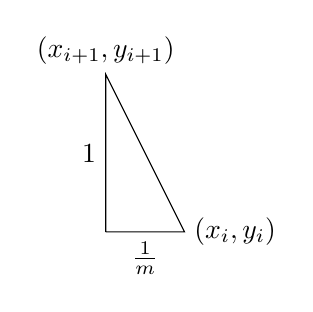
\begin{tikzpicture}[baseline=(current bounding box.north),x=10mm, y=10mm]
	\coordinate (A) at (0,0);
	\coordinate (B) at (1,0);
	\coordinate (C) at (0,2);
	\draw (A) -- (B) -- (C) -- (A);
	\path (B) node [right] {$(x_i,y_i)$};
	\path (C) node [above] {$(x_{i+1}, y_{i+1})$};
	\path (A) -- (B) node [midway, below] {$\frac{1}{m}$};
	\path (A) -- (C) node [midway, left] {1};
\end{tikzpicture}

\cr
\end{tabular}

\subsection{Color}

{\color{red}
	Notes on this section:  
	
	Make sure we're consistent about when to use $x_L - x_R$ and when to use $\lceil x_L \rceil - \lfloor x_R \rfloor$.
}

\

Computing color incrementally (Here considering only R, red)

Initialize $R_L = R_0$, $R_R = R_0$

For each scan line:

\

\qquad $\displaystyle R_L = R_L + \frac{R_1 - R_0}{y_1 - y_0}$

\

\qquad $\displaystyle R_R = R_R + \frac{R_2 - R_0}{y_2 - y_0}$

\

Within a scan line, between $\lceil x_L \rceil$ and $\lfloor  x_R \rfloor$

\



\qquad Initialize $\displaystyle R = R_L + \frac{R_L - R_R}{x_L - x_R} \left( \lceil x_L \rceil - x_L \right)$

\qquad Color first pixel

\qquad for $R$ from $R_L$ to $R_R$

\qquad \{

\qquad \qquad $\displaystyle R = R + \frac{R_L - R_R}{\lceil x_L \rceil - \lfloor x_R \rfloor } $

\qquad \qquad [Do the same for $G$ and $B$.]

\qquad \qquad Color pixel $(x, y, R, G, B)$

\qquad \}

\end{spacing}
\end{document}

%%%%%%%%%%%
%
% Useful code to recycle
%
%%%%%%%%%%

\hfil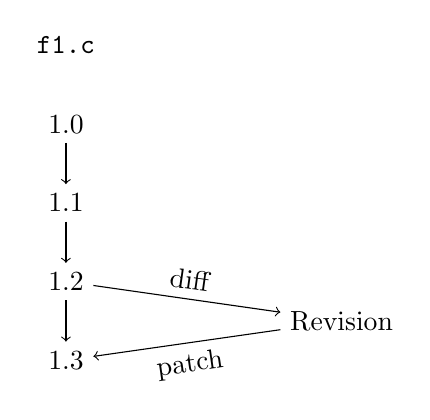
\begin{tikzpicture}
	[scale=0.5]
	\node (n0) at (0,0) {\tt f1.c};
	\node (n1) at (0,-2)  {1.0};
	\node (n2) at (0,-4)  {1.1};
	\node (n3) at (0,-6)  {1.2};
	\node (n4) at (0,-8)  {1.3};
	\node (n7) at (7,-7) {Revision};
  
	\foreach \from/\to in {n1/n2,n2/n3,n3/n4}
	\draw [->] (\from) -- (\to);

	\draw [->] (n3) -- node [above, sloped, midway] {diff} (n7);
	\draw [<-] (n4) -- node [below, sloped, midway] {patch} (n7);
\end{tikzpicture}









































